\documentclass[12pt]{article}

\usepackage[margin=1.9cm, letterpaper]{geometry}
\usepackage[utf8]{inputenc}
\usepackage{listings}
\usepackage{xcolor}
\usepackage{graphicx}
\usepackage{indentfirst}
\usepackage{tikz}
\usepackage{subcaption}
\usepackage{pdfpages}
\usepackage{mathtools}
\usepackage{hyperref}
\usepackage{siunitx}

\usepackage{parskip}
\setlength{\parskip}{1em}
\setlength{\parindent}{2em}

\usetikzlibrary{shapes.geometric, arrows}

\renewcommand{\thesection}{}
\renewcommand{\thesubsection}{}

\lstdefinestyle{mystyle}{
    basicstyle=\ttfamily\footnotesize,
    tabsize=4
}


\begin{document}
\begin{titlepage}
    \begin{center}
    \vspace*{1cm}
    
    \textbf{Lab 4}

    \vspace{0.5cm}

     Hardware Interfacing
    
    \vspace{1.5cm}

    \textbf{Hans Jarales (1537516) and Michael Kwok (1548454)}

    \vfill
            
    ECE 212 Lab - Introduction to Microprocessors\\
    Department of Electrical and Computer Engineering\\
    University of Alberta\\
    Apr.8, 2020   

   \end{center}
\end{titlepage}

\section{Free-Form Report:}
This lab explores hardware interfacing using a Netburner and buffer board to communicate with an 8x8 LED array. Two 3x8 74LS138 decoders, two hex-input 74LS04 inverters and 8 \SI{1}{\kilo\ohm} resistors are additionally used. It shows how software and hardware can be used to do things that are basically impossible with only software, and really difficult with just hardware.

A 10-pin ribbon cable is used to communicate data from the Netburner pins, to the buffer board, and ultimately to the breadboard containing the IC/LED array circuit. Output Pins 37-43 of the Netburner are mapped to the 10-pin ribbon cable of the buffer board, more specifically, pins 1-7, where pin 8 is not used, and pin 9 and 10 are for ground/power source connections.

The WelcomePrompt subroutine prompts the user to enter a single character -- the character being a number or uppercase letter. An invalid character results in re-prompting the user for proper input. The character, stored in ASCII, is placed in the stack, where it is passed onto the Convert subroutine. Here, the address of the pattern based on the input character is passed onto the stack. The pattern is stored as 2 Longword-sized data content, corresponding to an 8x8 array. The following is an example of how the letter A is stored in memory (taken from pattern.s):

\begin{verbatim}
.data
Letter_A:
.byte 0b00011000        /* This is the pattern for the letter A */
.byte 0b00100100        /* A bit '1' indicates an activated LED in the 8x8 LED Array */
.byte 0b01000010        /* A bit '0' indicates an inactive LED */
.byte 0b01111110
.byte 0b01000010        /* A user input of 'A' will result in convert1 taking the */
.byte 0b01000010        /* address of this pattern in the Convert subroutine */
.byte 0b01000010
.byte 0b01000010        
\end{verbatim}

The LedSub subroutine uses the pattern address passed from the stack to display the pattern based on the user input, which has the address of the pattern of which is stored in the stack. Every row and column in the pattern is checked to see if the LED has to be switched on or off, then switched accordingly; 1 for on and 0 for off. After the entire array has been iterated over, the subroutine runs a 300 unit delay before returning from the subroutine to allow for visible time with the LEDs.

\begin{figure}
    \centering
    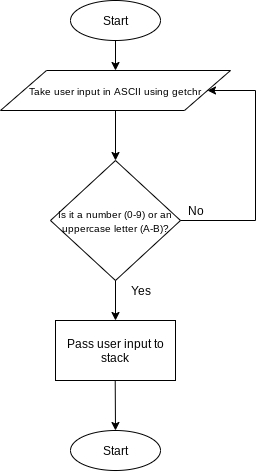
\includegraphics[scale=0.5]{Lab4/Lab4a.png}
    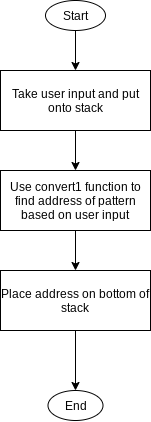
\includegraphics[scale=0.5]{Lab4/Lab4b.png}
    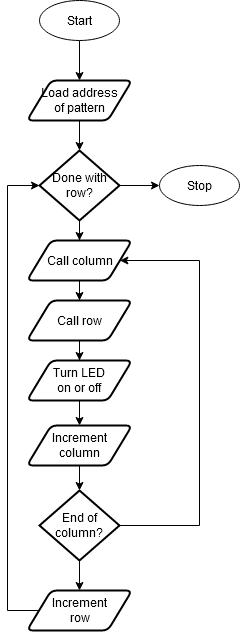
\includegraphics[scale=0.5]{Lab4/Lab4c.png}
    \caption{Flowcharts}
\end{figure}

\section{Question}
Why were the two 74LS138 decoders used in the circuit instead of directly connecting the pins to the array? Discuss how removing the decoders would affect the function of the LED array in the context of this lab.

Since we are using an 8x8 LED array, the minimum number of bits that are needed to represent each axis is 3 bits ($\log_2(8) = 3$). To differentiate between the row and column LED activations, the two 3x8 74LS138 decoders are used -- where the 74LS138 utilizes 3 Address input pins and produces an 8-bit output to determine the row or column being activated. Since the LED array requires a one-hot input to enable the LEDs and not a binary number, the decoder is used. If we did not use the decoder, we would need 16 pins from the board to output to the matrix, 8 for each axis. This way we could utilize the pins on the board for other uses such as more LED matrices if we need or different peripherals.

If the decoders were not used, we would need a wider connector from the development board to the buffer board that could carry 16 bits instead of 10, so that we would be able to select the LEDs directly from the microprocessor. We would also have to modify the TurnOnLed and TurnOffLed subroutines to select the correct new pins.

\end{document}